\section{Вычислительный эксперимент} \label{section:experiments}

В этом разделе представлены численные эксперименты с глубокими нейронными сетями, которые направлены на глубокий анализ новых методов сжатия и исследование их влияния на сходимость.

\subsection{Детали реализации}
    Современные глубокие нейронные сети состоят из большого количества слоев с различными характеристиками. Это естественным образом поднимает вопрос: как следует выбирать координаты, учитывая неоднородность весов? В наших экспериментах мы фиксируем коэффициент сжатия $\alpha = k/d$, где $k$ — количество выбранных координат, а $d$ — общее количество параметров в нейронной сети (в наших экспериментах установлено на уровне 1\%). Затем мы применяем оператор сжатия к градиентам каждого слоя, выбирая $k_i = \lceil \alpha \cdot d_i \rceil$ координат в $i$-м слое размером $d_i$. Полученный тензор размером $d_i$ содержит $k_i$ ненулевых координат, которые передаются оптимизатору. Кроме того, могут быть использованы методы компенсации ошибок, в этом случае оператор применяется к градиенту с добавленной накопленной ошибкой. Такой выбор координат по слоям позволяет более равномерно сравнивать группы весов.

    Теперь о вычислении $w$ для слоев нейронной сети. В начале каждой эпохи мы решаем задачу
    \begin{equation}
        \argmin_{w \in \{x \cdot d | x \in \Delta_{d_i - 1}\}} f(x - \eta w \odot \nabla f(x))
    \end{equation}
    в случае $\impk_s$ и 
    \begin{equation}
        \argmin_{w \in [0,2]^{d_i}} f(x - \eta w \odot \nabla f(x))
    \end{equation}
    в случае $\impk_c$. Для решения этих задач мы используем метод зеркального спуска на симплексе и градиентный спуск на кубе соответственно. Начальная точка для $w$ выбирается как вектор из единиц, что соответствует методу $\topk$. Для повышения вычислительной эффективности мы используем небольшое количество итераций и большой шаг $\eta$, и все значения важности $w$ обновляются одновременно.

    Кроме того, методы на основе $\impk$ используют значения $w$ не только для выбора координат градиента, но и для их перенормировки. В частности, действие компрессора $\impk$ можно выразить следующей формулой:
    \begin{align*}
        \impk(\nabla f(x)) = \sum_{i=1}^{k_i} (w \odot \nabla f(x))_{(i)} e_{(i)},
    \end{align*}
    где $k_i$ координат выбираются в порядке убывания $|w_i \cdot \nabla f(x)_i|$. 
    В методах с обратной связью по ошибке для выбора координат и сжатия используется градиент с накопленной ошибкой $\nabla f(x) + \varepsilon$, где $\varepsilon$ представляет накопленную ошибку.

    Метод SCAM сочетает оба подхода: выбор координат выполняется в порядке убывания $|(w \odot (\nabla f(x) + \varepsilon))_i|$, и возвращается перенормированный градиент без ошибки:
    \begin{align*}
        \impk(\nabla f(x)) = \sum_{i=1}^{k_i} (w \odot \nabla f(x))_{(i)} e_{(i)}.
    \end{align*}

\subsection{Техническая информация}
    Эксперименты по обучению ResNet-18 проводились на GPU NVIDIA GeForce RTX 2080 Ti с 12 ГБ видеопамяти, при этом 50 эпох обучения занимали примерно 25 минут. Для обучения GPT-2 на датасете WikiText2 использовался GPU NVIDIA A100 с 40 ГБ видеопамяти, и 50 эпох обучения занимали примерно 2 часа.

\subsection{Сверточные нейронные сети}

    В контексте решения задачи CIFAR-10 было принято решение использовать архитектуру ResNet-18, которая получила значительное распространение в соответствующей экспериментальной среде. Был проведен ряд экспериментов с целью выяснить различия и улучшения, которые могут быть достигнуты с использованием современных компрессоров. <<Качество>> методов исследуется через сравнение с $\topk$ и его модификацией с обратной связью по ошибке. В ходе исследования предполагается, что размер батча будет установлен на уровне 128, а данные будут случайным образом распределены между ними.

    Теперь мы переходим к оценке производительности вновь предложенного семейства операторов сжатия в процессе обучения. В частности, мы рассматриваем задачу обучения модели ResNet-18 на датасете CIFAR-10. В качестве оптимизатора был выбран CAdamW со следующими гиперпараметрами: $\beta_1 = 0.9, \beta_2 = 0.999$ и коэффициентом затухания весов, установленным на $0.01$. Это AdamW с сжатием: он использует сжатый градиент вместо оригинального. Коэффициент сжатия был зафиксирован на уровне 1\%. Скорость обучения была оптимально настроена для каждого компрессора, обычно в диапазоне от $0.0001$ до $0.002$. Количество эпох обучения составляет $50$. Результаты запусков усреднялись по 5 различным начальным значениям. Графики отображают средние значения вместе с выборочной дисперсией.
    \begin{figure}[ht]
        \centering
            \textbf{Эксперимент 1}\par\medskip
            \begin{minipage}{0.45\textwidth}
                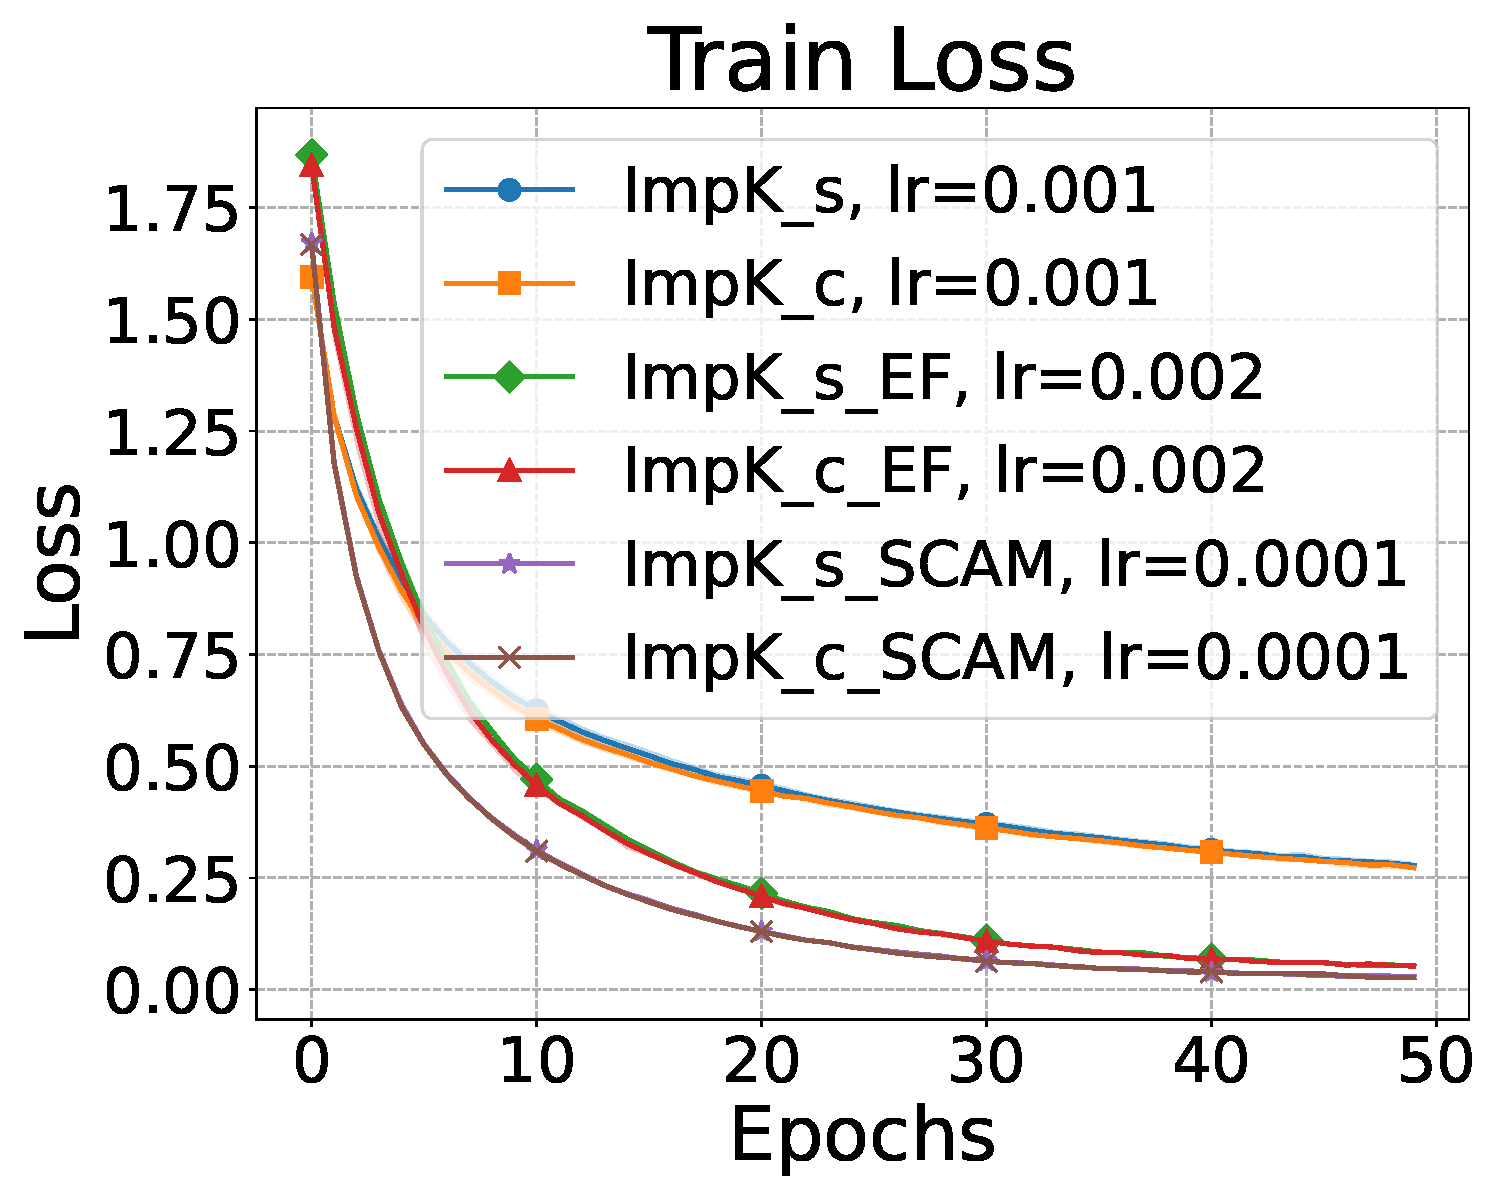
\includegraphics[width=\textwidth]{figures/resnet/experiment1/Train Loss.pdf}
            \end{minipage}
            \begin{minipage}{0.45\textwidth}
                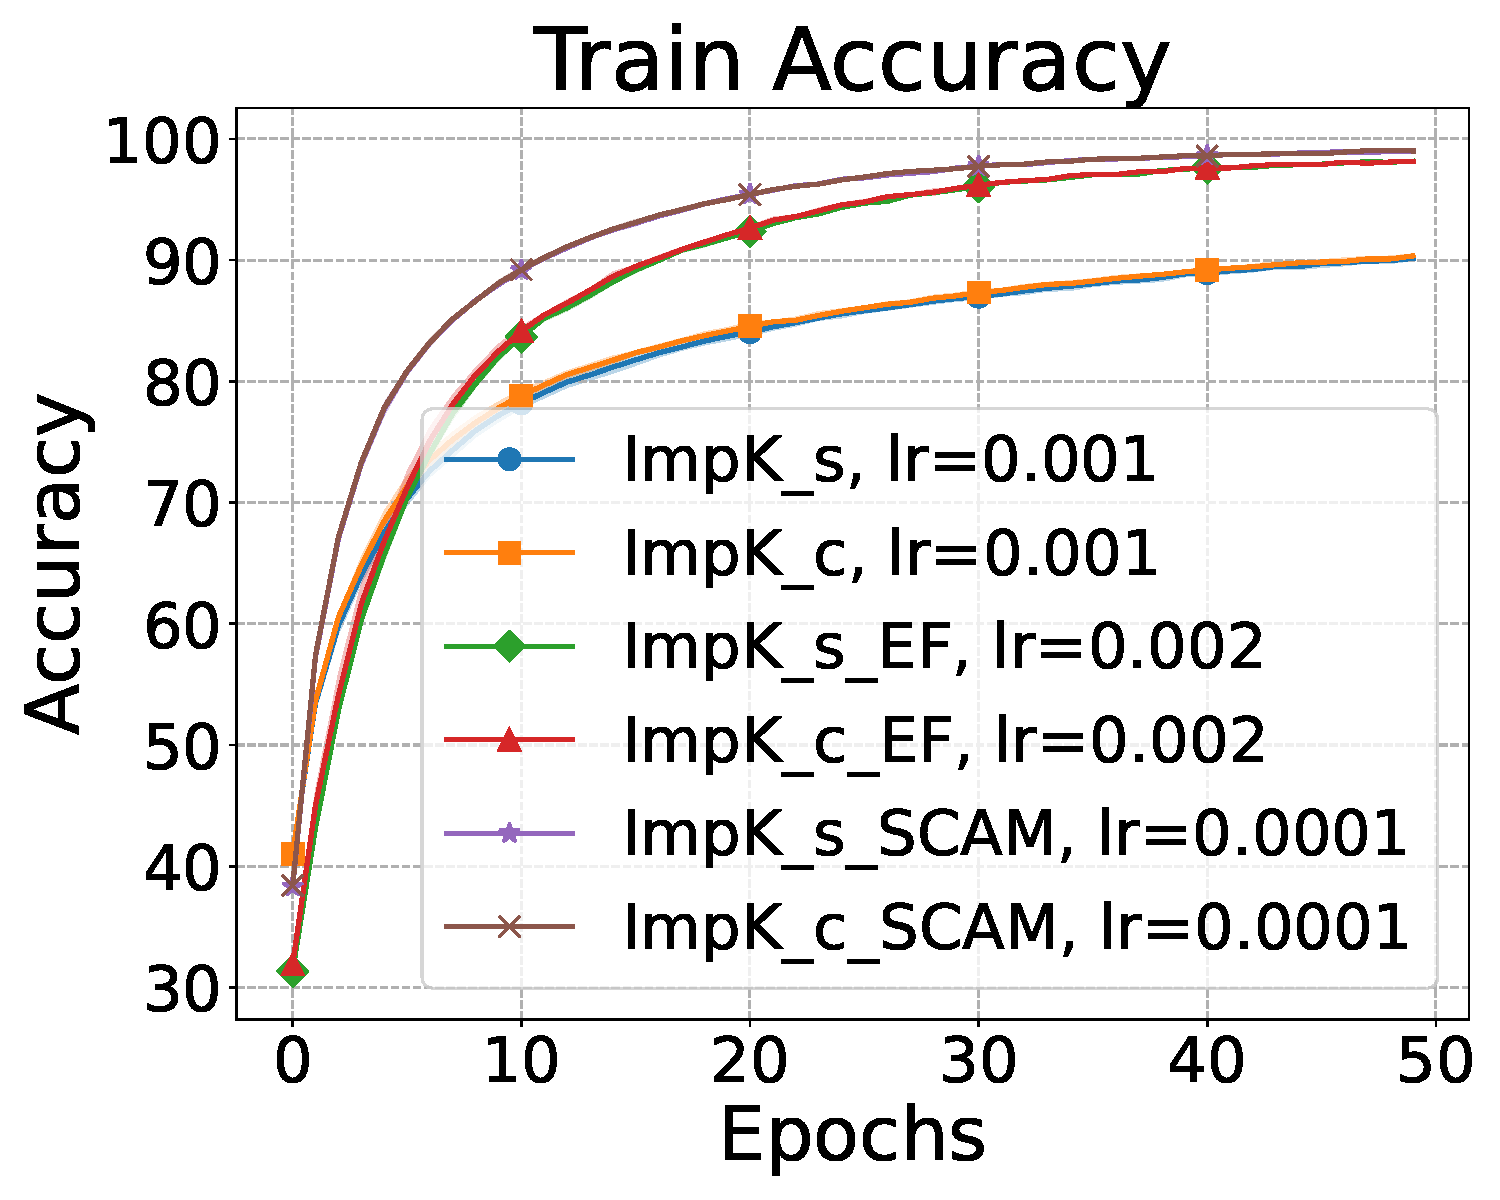
\includegraphics[width=\textwidth]{figures/resnet/experiment1/Train Accuracy.pdf}
            \end{minipage}
            \begin{minipage}{0.45\textwidth}
                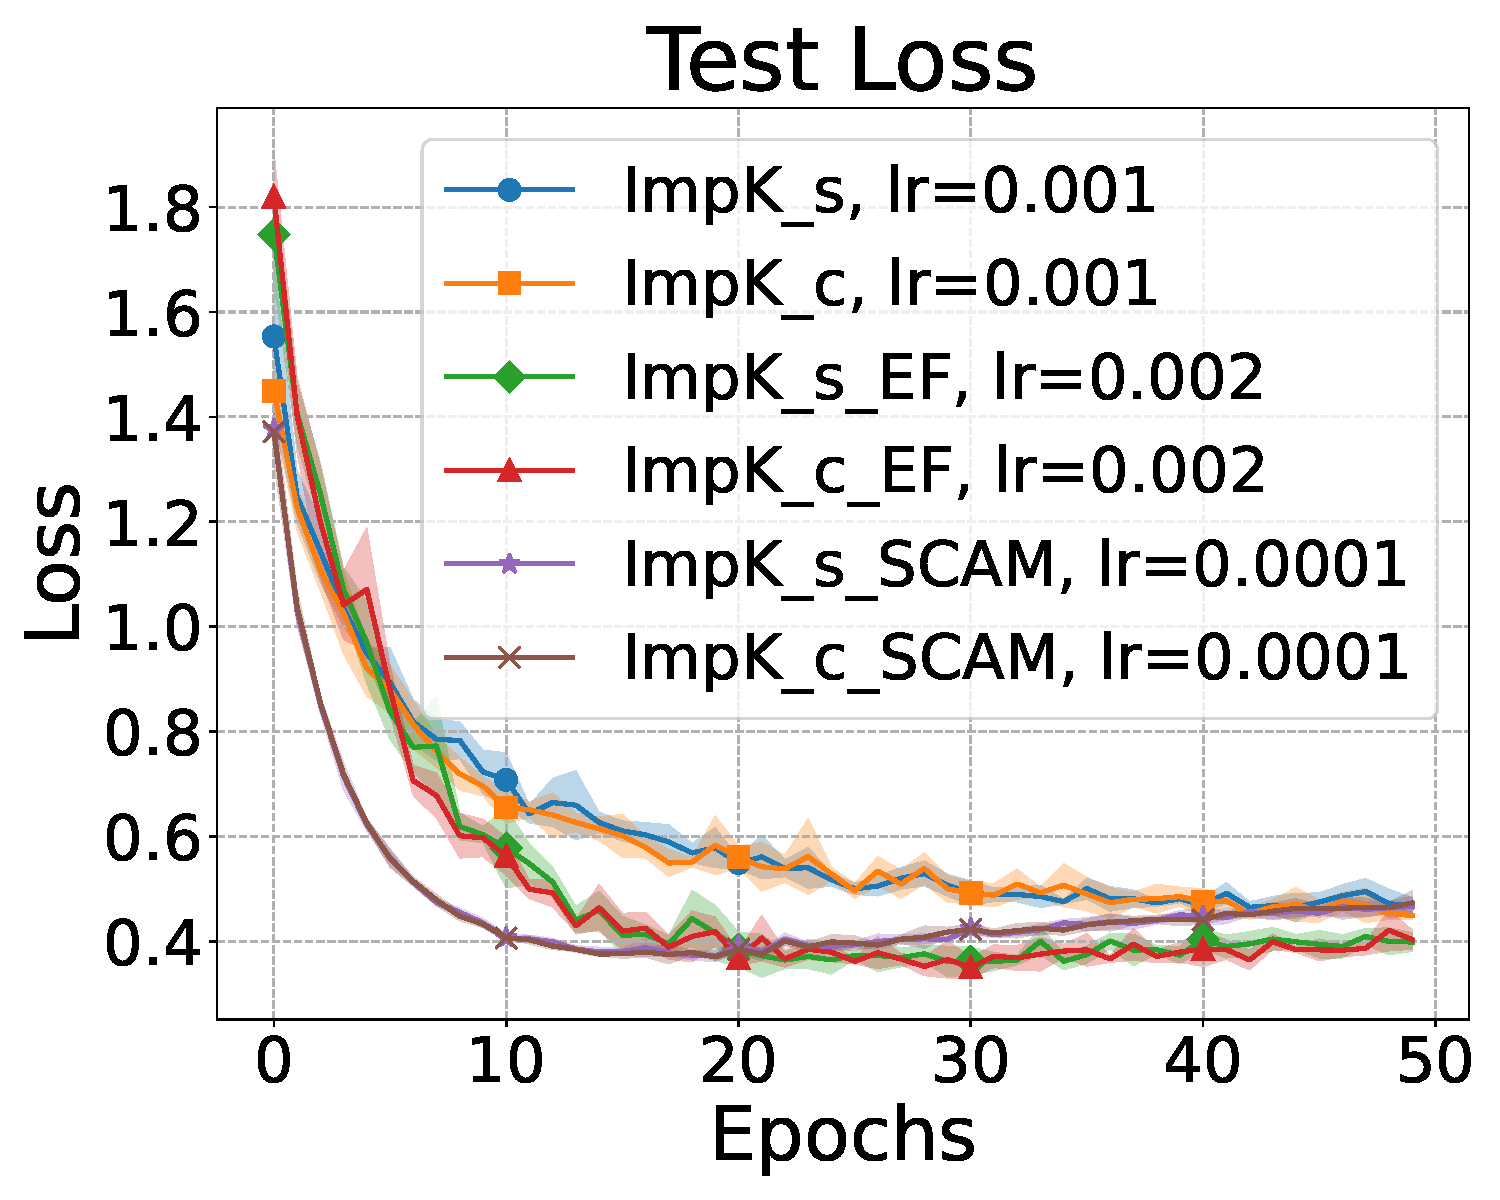
\includegraphics[width=\textwidth]{figures/resnet/experiment1/Test Loss.pdf}
            \end{minipage}
            \begin{minipage}{0.45\textwidth}
                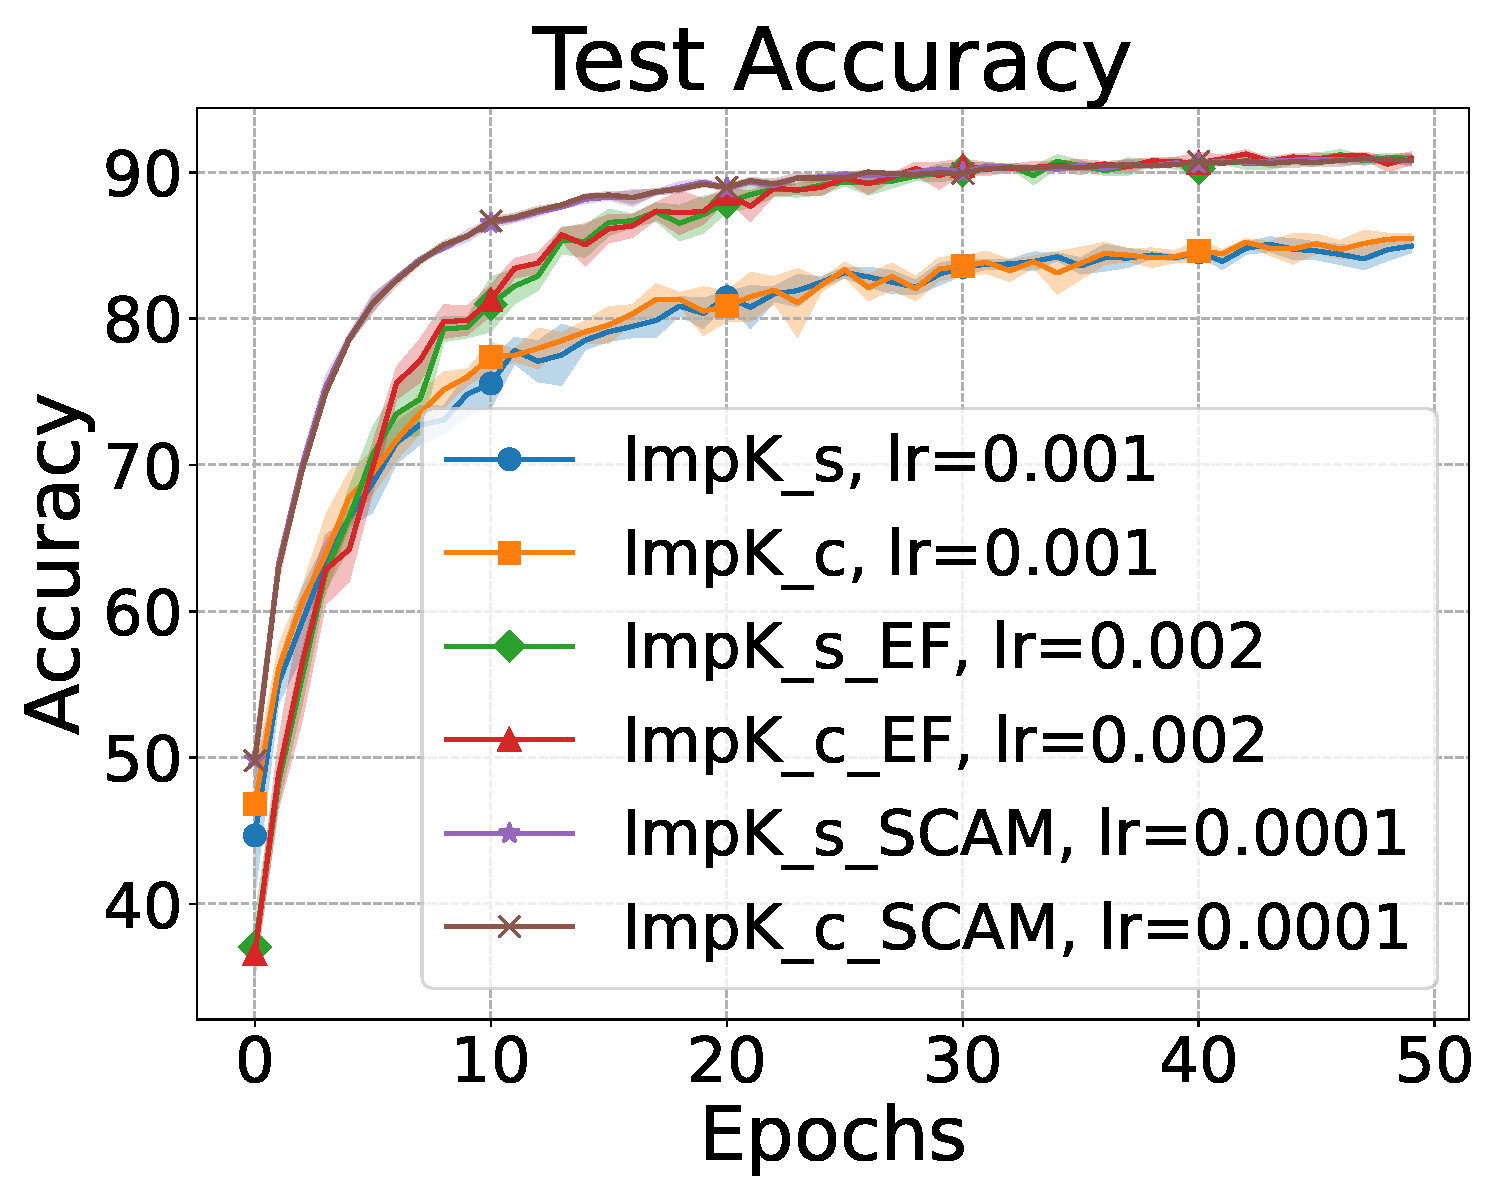
\includegraphics[width=\textwidth]{figures/resnet/experiment1/Test Accuracy.pdf}
            \end{minipage}
            \caption{Сравнение производительности предложенных методов сжатия в процессе обучения ResNet-18 на датасете CIFAR-10.}
    \end{figure}
    На основе графиков можно сделать вывод, что в этой задаче методы SCAM $\impk_s$ и SCAM $\impk_c$ показывают лучшие результаты. Они сходятся быстрее и точнее по сравнению с другими методами. В следующем эксперименте мы сравниваем лучший метод из нашего семейства с явным базовым вариантом в виде вариаций $\topk$. Для простоты мы выбираем SCAM $\impk_c$, так как он менее чувствителен к настройке гиперпараметров и менее подвержен расходимости. Мы сравниваем его с $\topk$ без коррекции ошибок, $\topk$ с техникой обратной связи по ошибке, а также с техникой SCAM, адаптированной для $\topk$.
    \begin{figure}[ht]
        \centering
        \textbf{Эксперимент 2}\par\medskip
        \begin{minipage}{0.45\textwidth}
            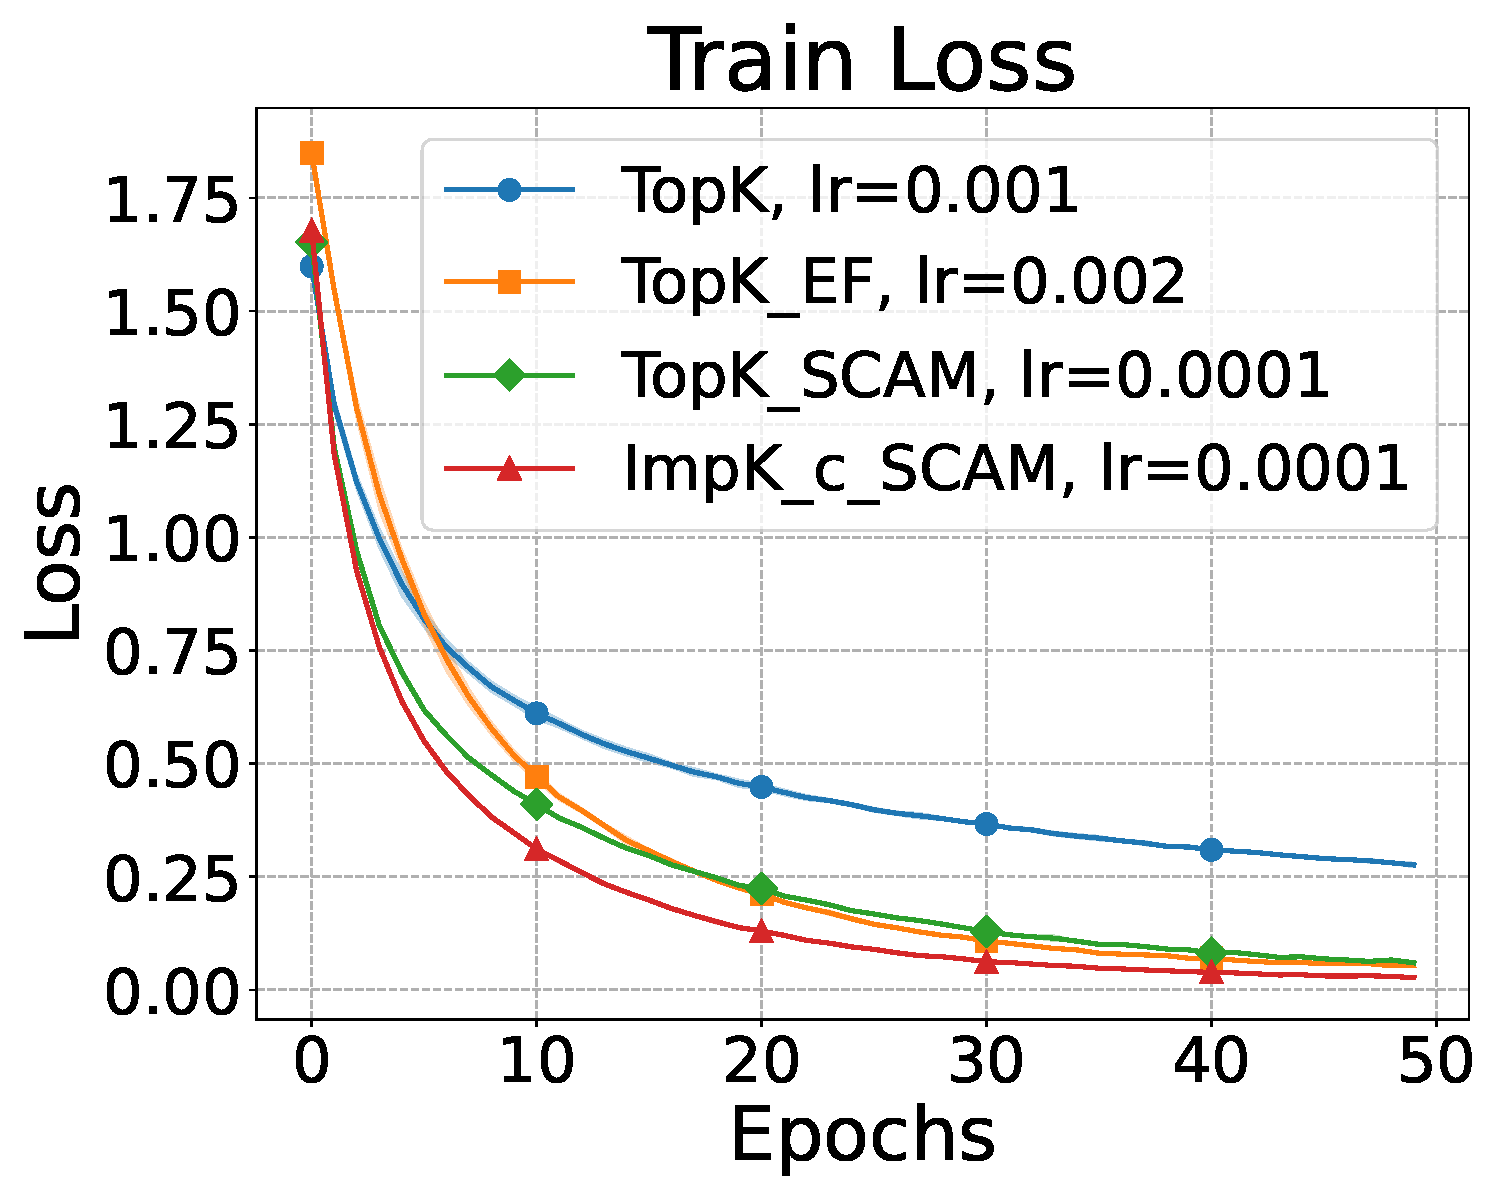
\includegraphics[width=\textwidth]{figures/resnet/experiment2/Train Loss.pdf}
        \end{minipage}
        \begin{minipage}{0.45\textwidth}
            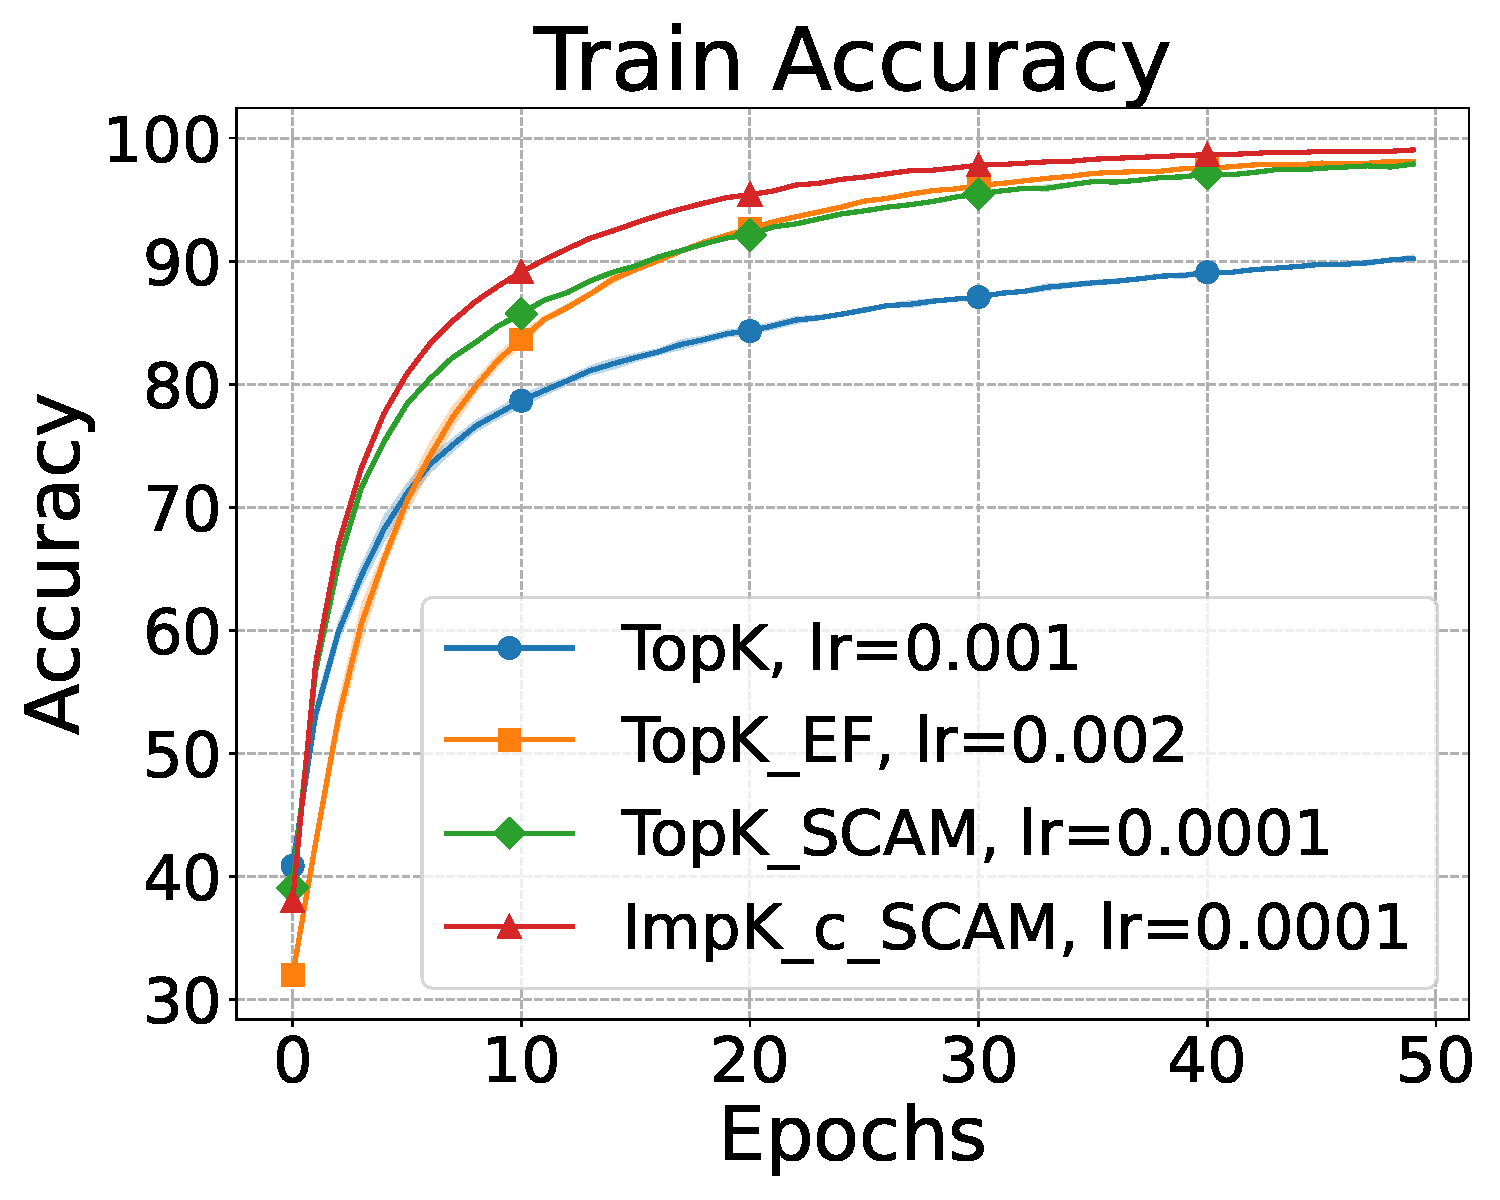
\includegraphics[width=\textwidth]{figures/resnet/experiment2/Train Accuracy.pdf}
        \end{minipage}
        \begin{minipage}{0.45\textwidth}
            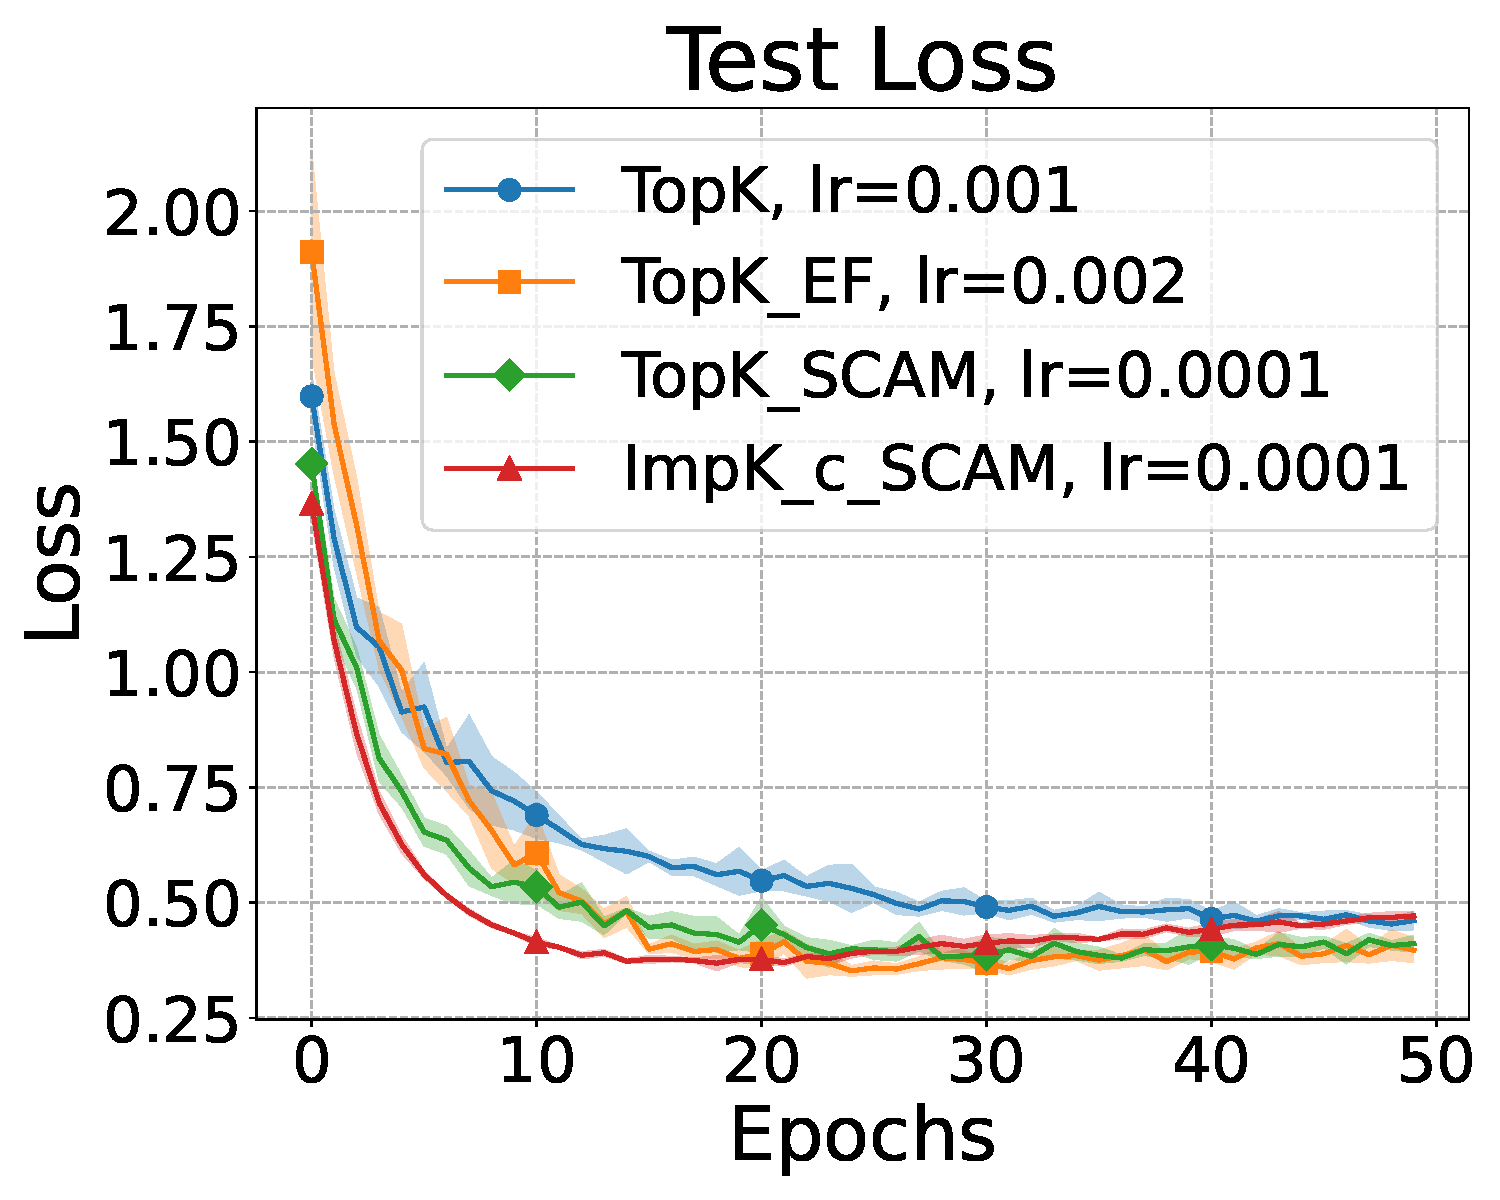
\includegraphics[width=\textwidth]{figures/resnet/experiment2/Test Loss.pdf}
        \end{minipage}
        \begin{minipage}{0.45\textwidth}
            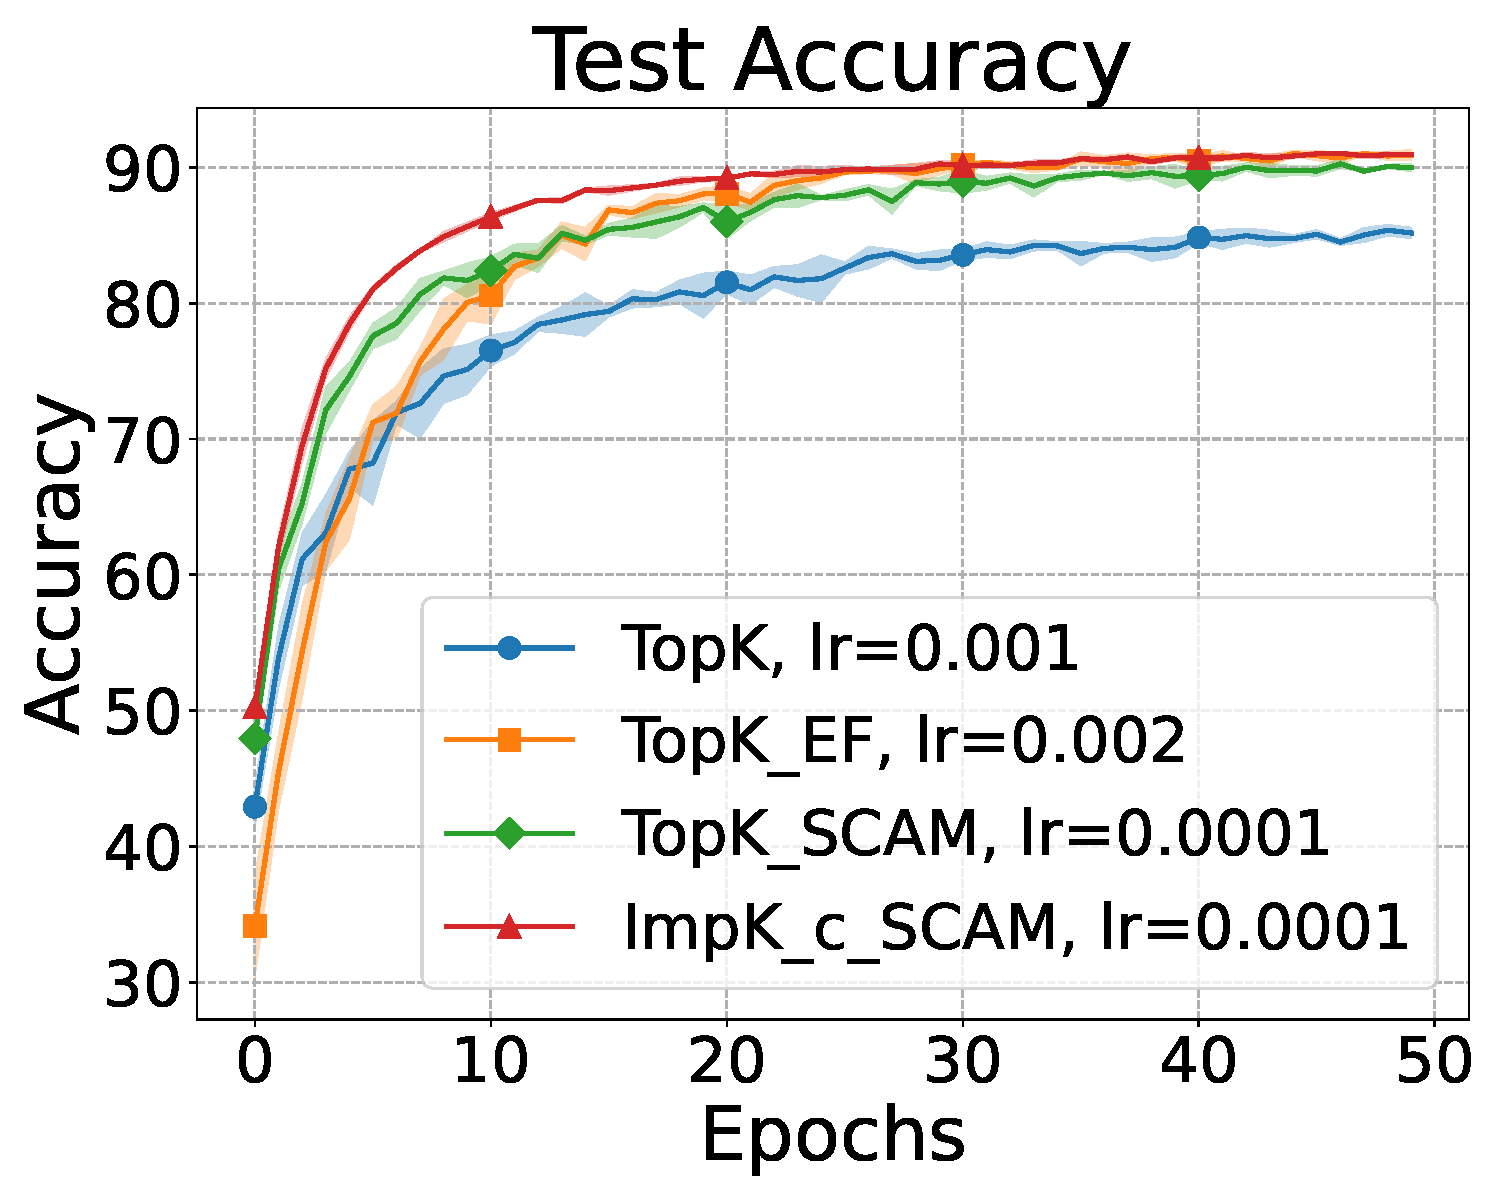
\includegraphics[width=\textwidth]{figures/resnet/experiment2/Test Accuracy.pdf}
        \end{minipage}
        \caption{Сравнение производительности между предложенным методом SCAM $\impk_c$ и вариациями $\topk$ в процессе обучения ResNet-18 на датасете CIFAR-10.}
    \end{figure}
    Анализ графиков демонстрирует, что техника SCAM в сочетании с предложенным оператором сжатия $\impk_c$ превосходит все методы, использующие $\topk$. Адаптация SCAM для $\topk$ показывает более высокую скорость сходимости в начале обучения, но начинает отставать от обратной связи по ошибке примерно на 20-й эпохе.

    Затраты на решение задачи минимизации один раз за эпоху составляют примерно 10\% времени обучения, что компенсируется достигнутым ускорением.

\subsection{Трансформерная архитектура}
    В этом подразделе в качестве базовой модели для экспериментов использовалась языковая модель GPT-2 Small (124M). Модель была инициализирована случайным образом с конфигурацией, соответствующей предобученному токенайзеру GPT-2, датасет — WikiText2, разделенный на обучающую и валидационную части. Размер батча был установлен на уровне $16$, каждая последовательность токенов в батче имеет длину $1024$.

    Оптимизатор остается CAdamW с теми же гиперпараметрами. Скорость обучения была оптимально настроена для каждого компрессора, варьируясь от $0.0001$ до $0.001$. Количество эпох обучения составляет $50$.

    Мы проведем два эксперимента, следуя методике из предыдущего подраздела. Снова сравним методы на основе $\impk$ друг с другом.

    % GPT-2 on WikiText2: Experiment 1 (4 plots)
    \begin{figure}[ht]
        \centering
        \textbf{Эксперимент 1}\par\medskip
        \begin{minipage}{0.45\textwidth}
            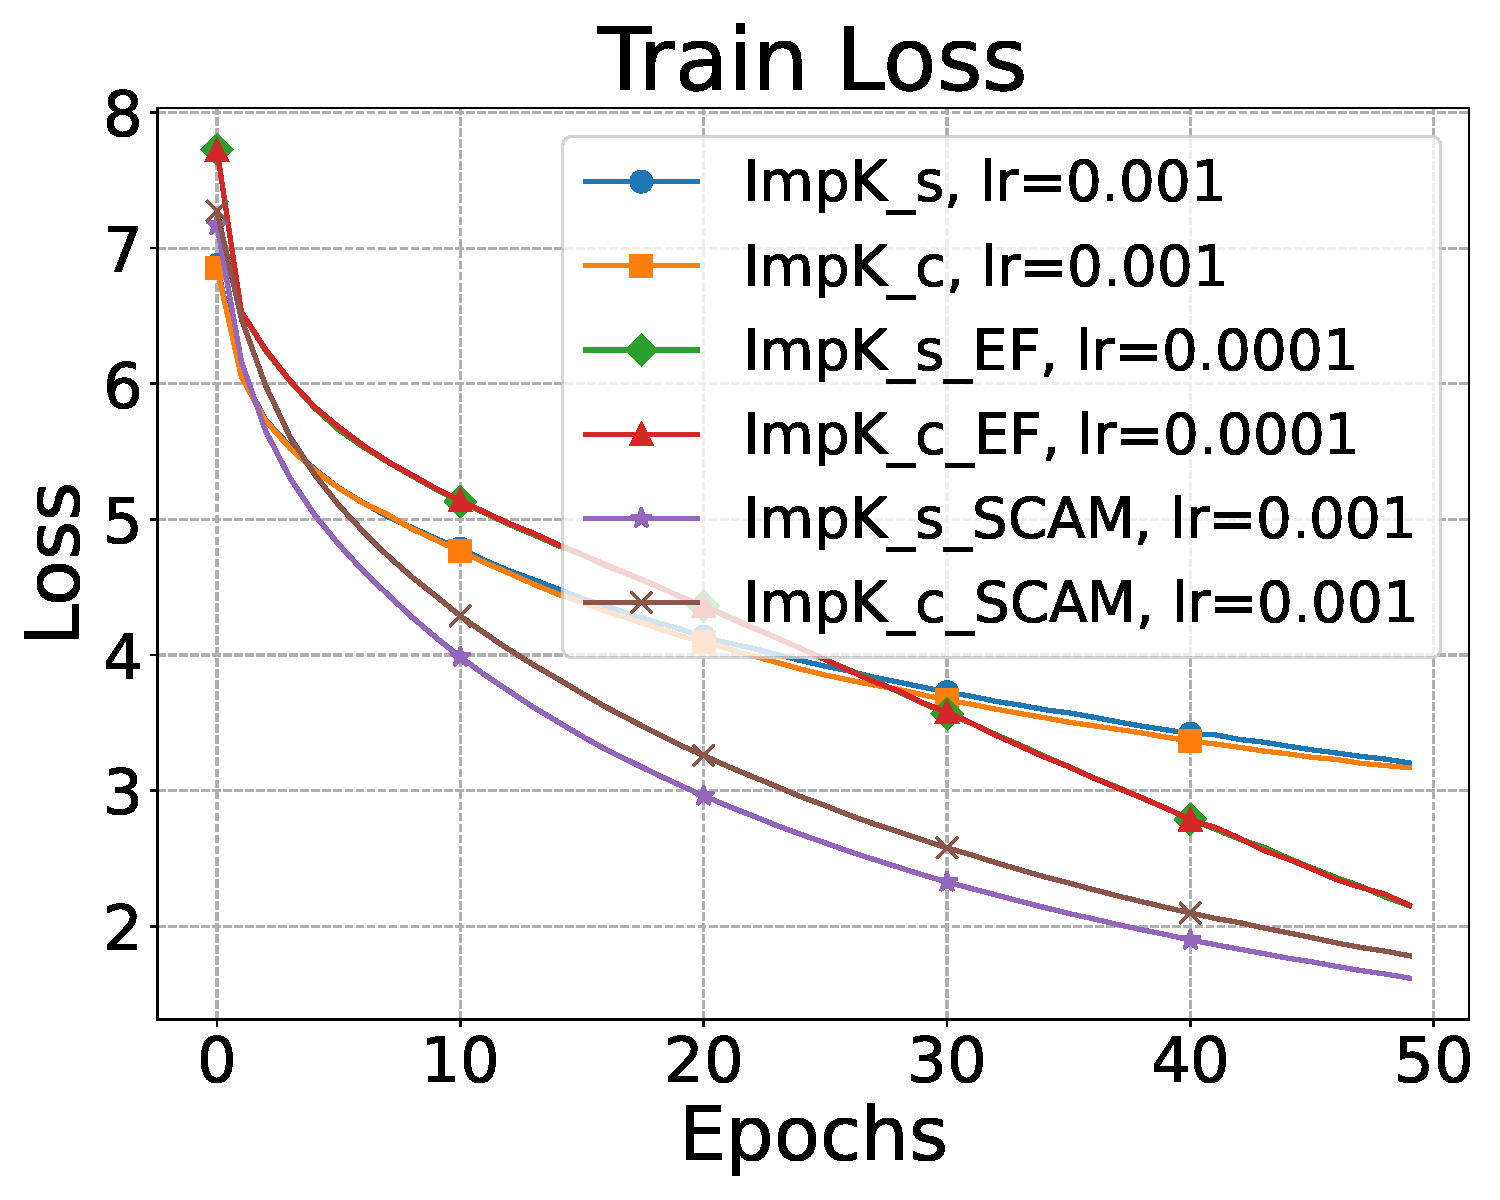
\includegraphics[width=\textwidth]{figures/gpt2/experiment1/Train Loss.pdf}
        \end{minipage}
        \begin{minipage}{0.45\textwidth}
            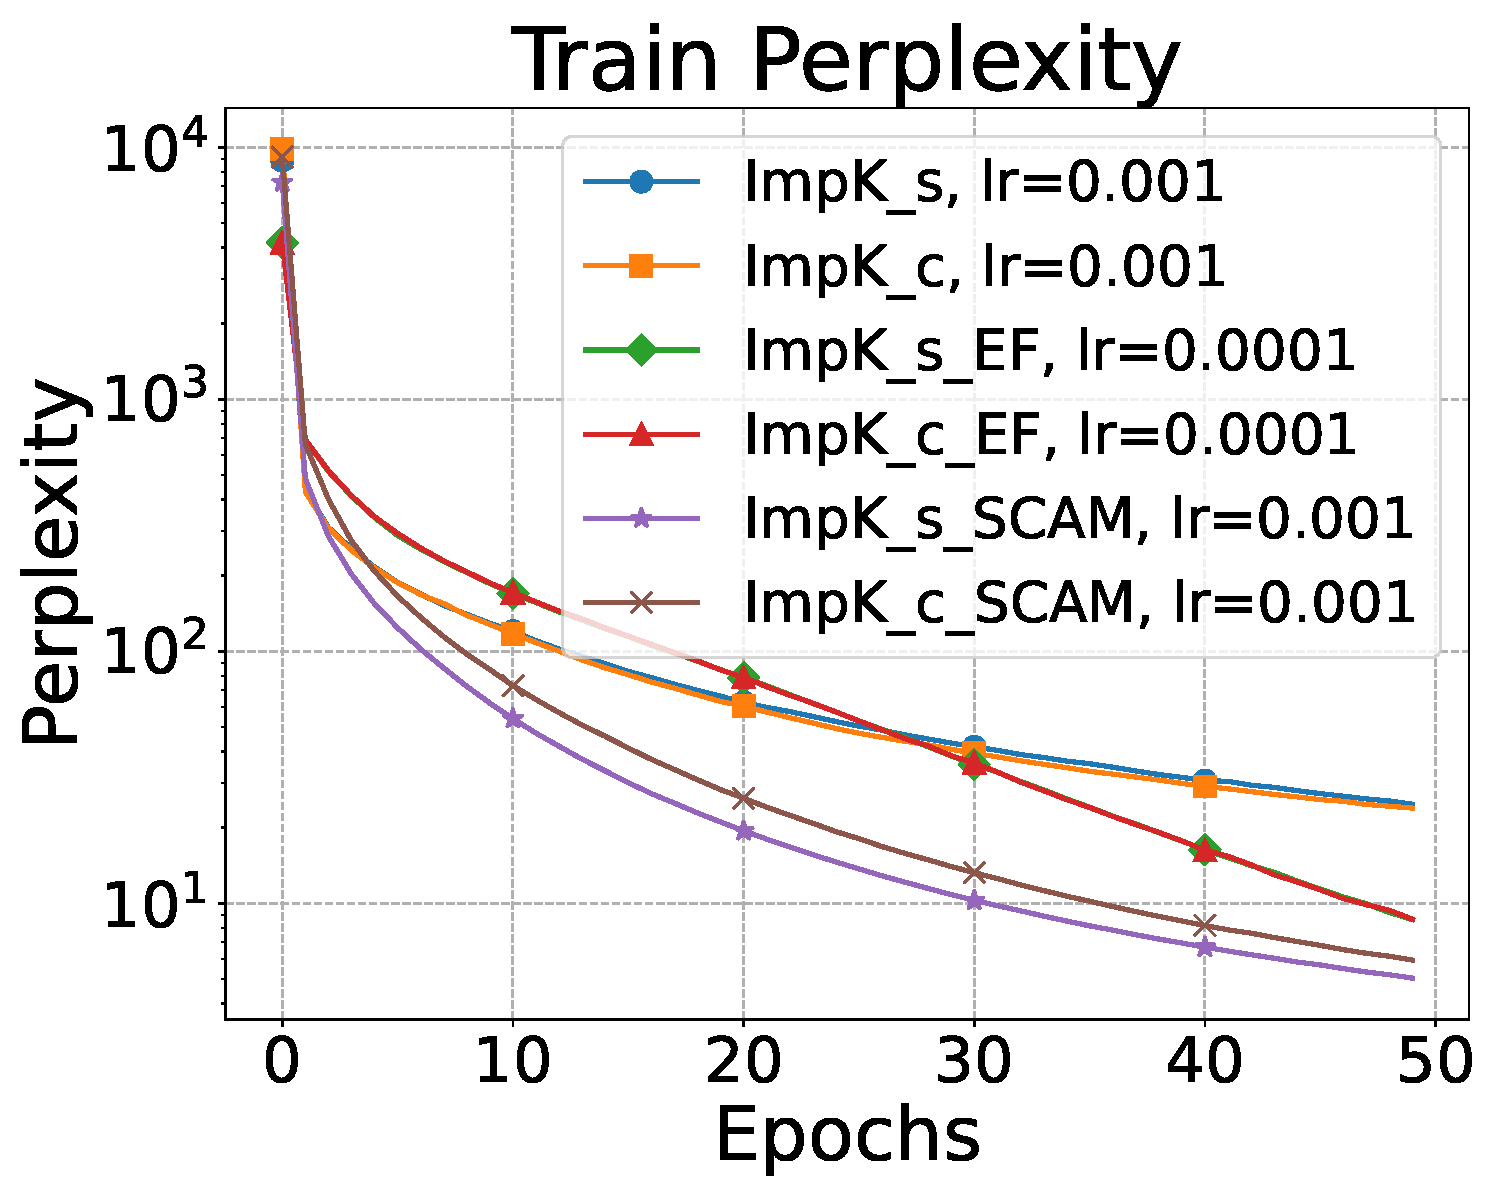
\includegraphics[width=\textwidth]{figures/gpt2/experiment1/Train Perplexity.pdf}
        \end{minipage}
        \begin{minipage}{0.45\textwidth}
            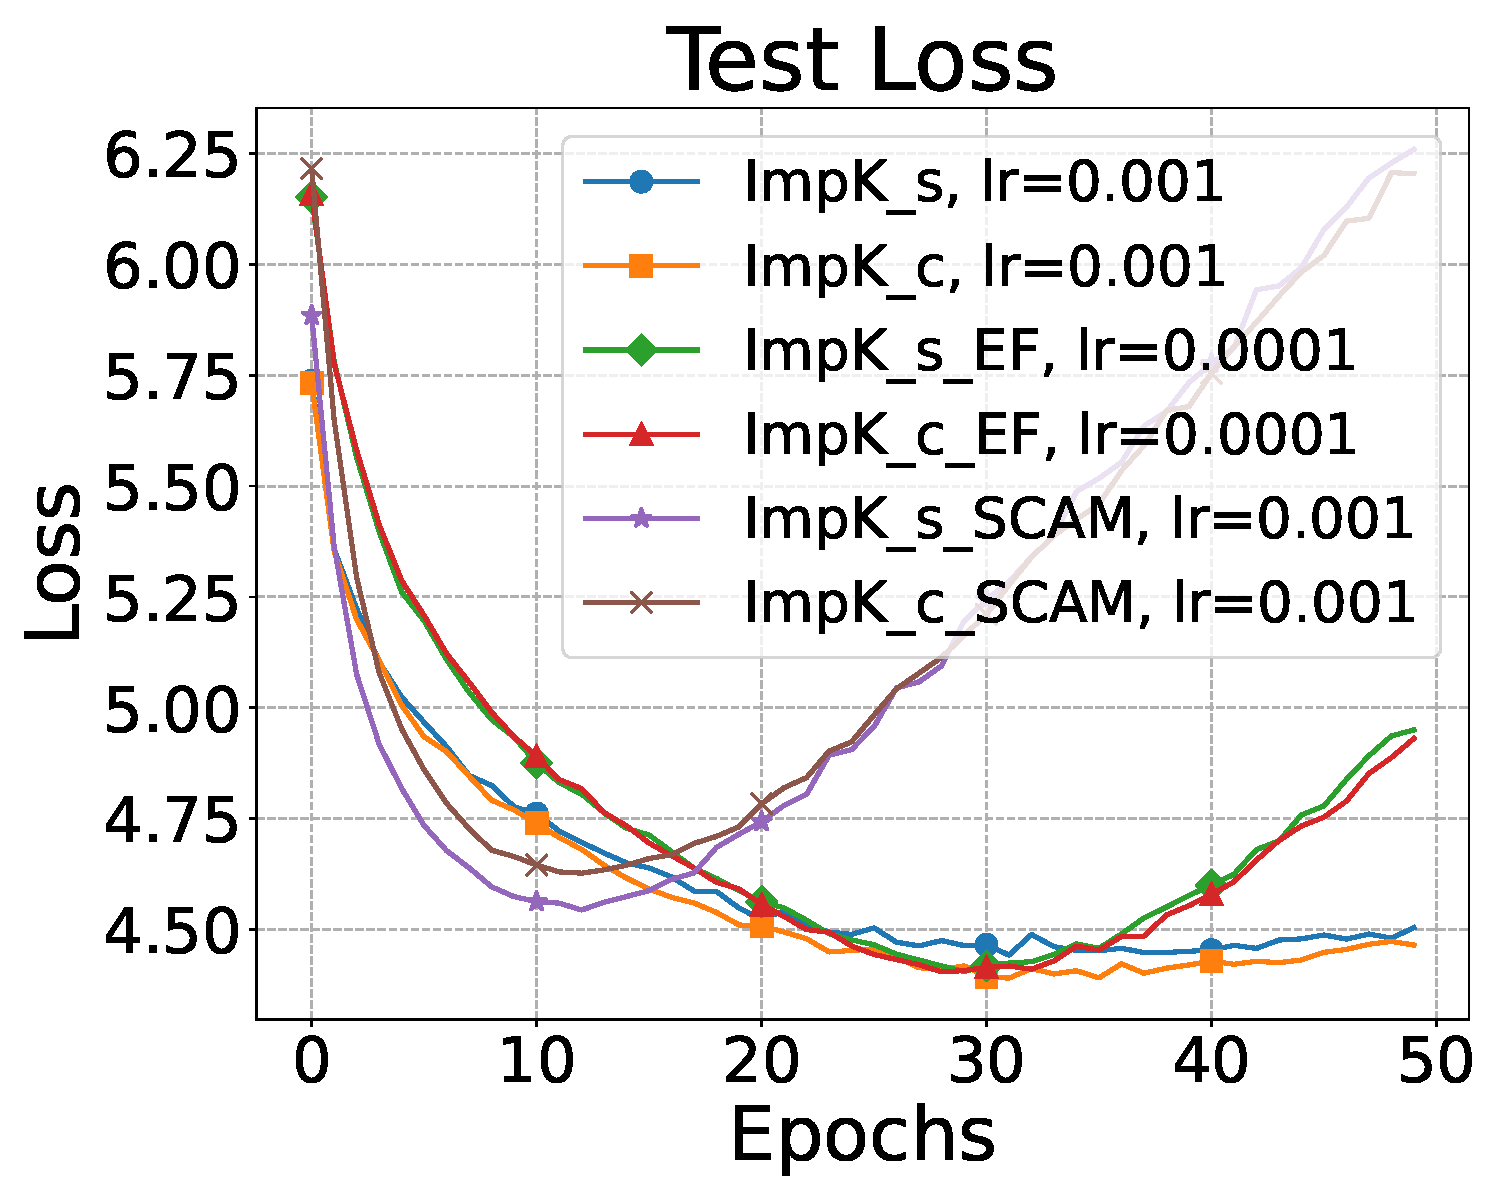
\includegraphics[width=\textwidth]{figures/gpt2/experiment1/Test Loss.pdf}
        \end{minipage}
        \begin{minipage}{0.45\textwidth}
            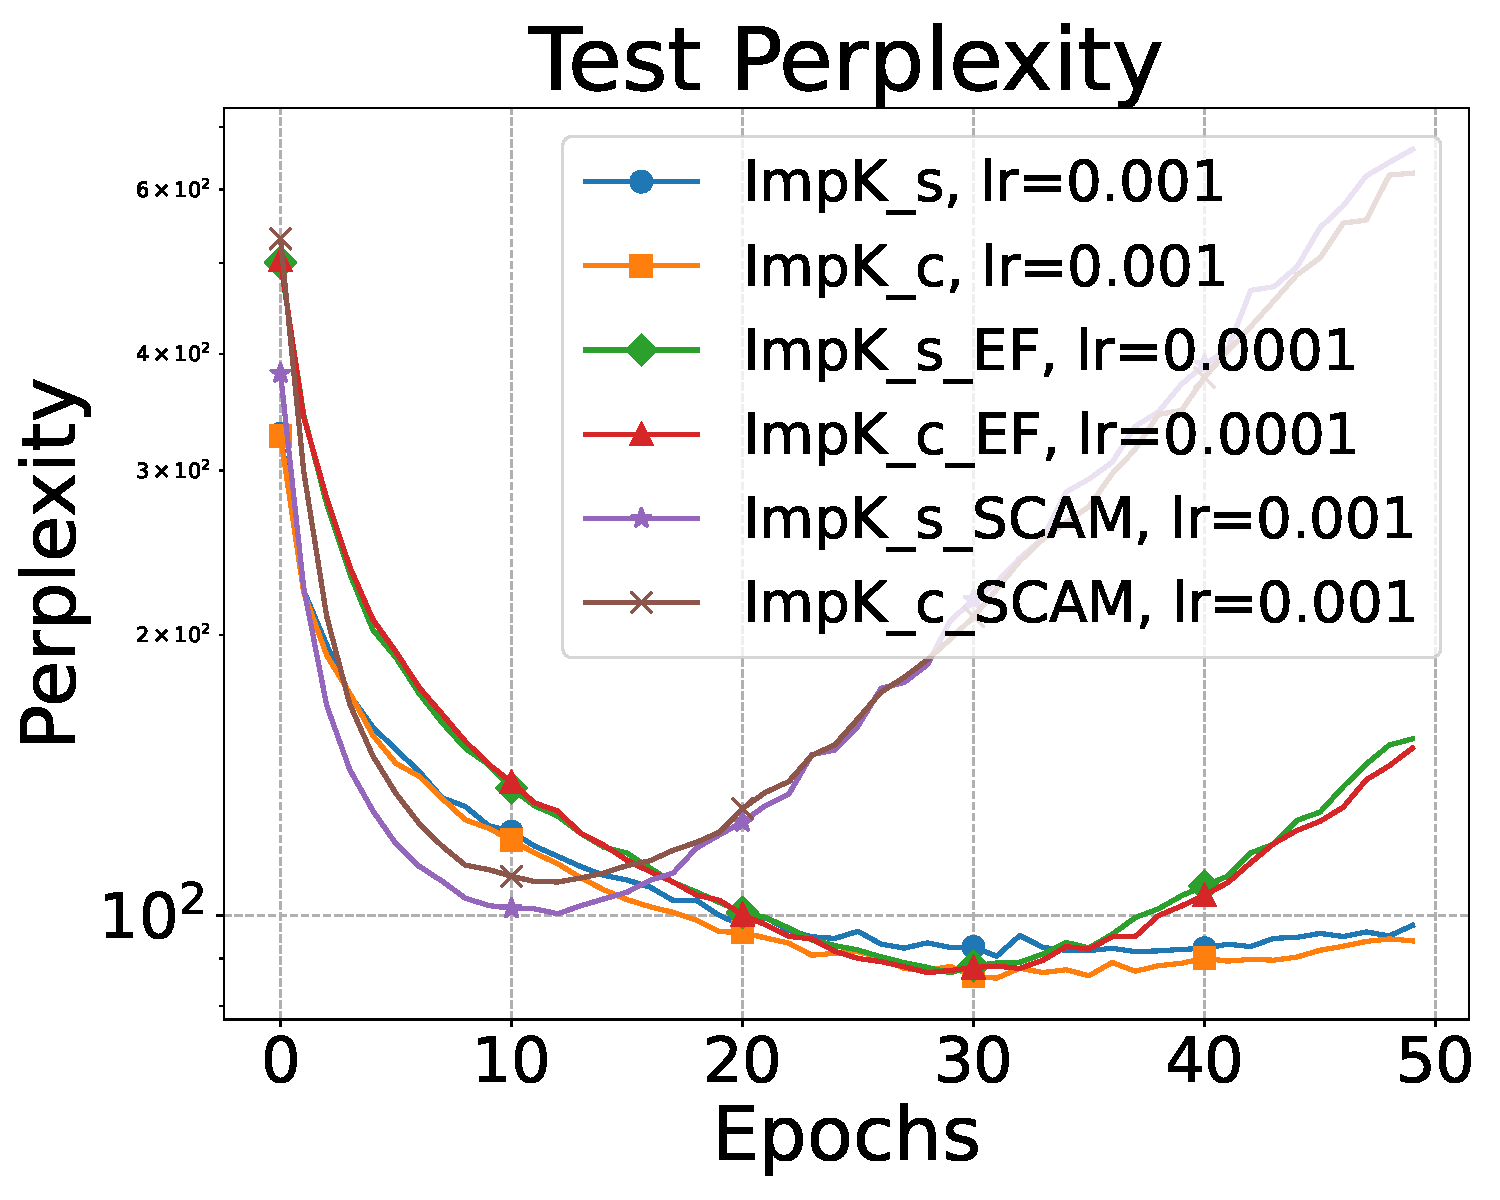
\includegraphics[width=\textwidth]{figures/gpt2/experiment1/Test Perplexity.pdf}
        \end{minipage}
        \caption{Сравнение производительности предложенных методов сжатия в процессе обучения GPT-2 на WikiText2.}
    \end{figure}

    Для второго эксперимента мы выбираем лучший метод для решения задачи, SCAM $\impk_s$, и сравниваем его с методами на основе $\topk$.

    % GPT-2 on WikiText2: Experiment 2 (4 plots)
    \begin{figure}[ht]
        \centering
        \textbf{Эксперимент 2}\par\medskip
        \begin{minipage}{0.45\textwidth}
            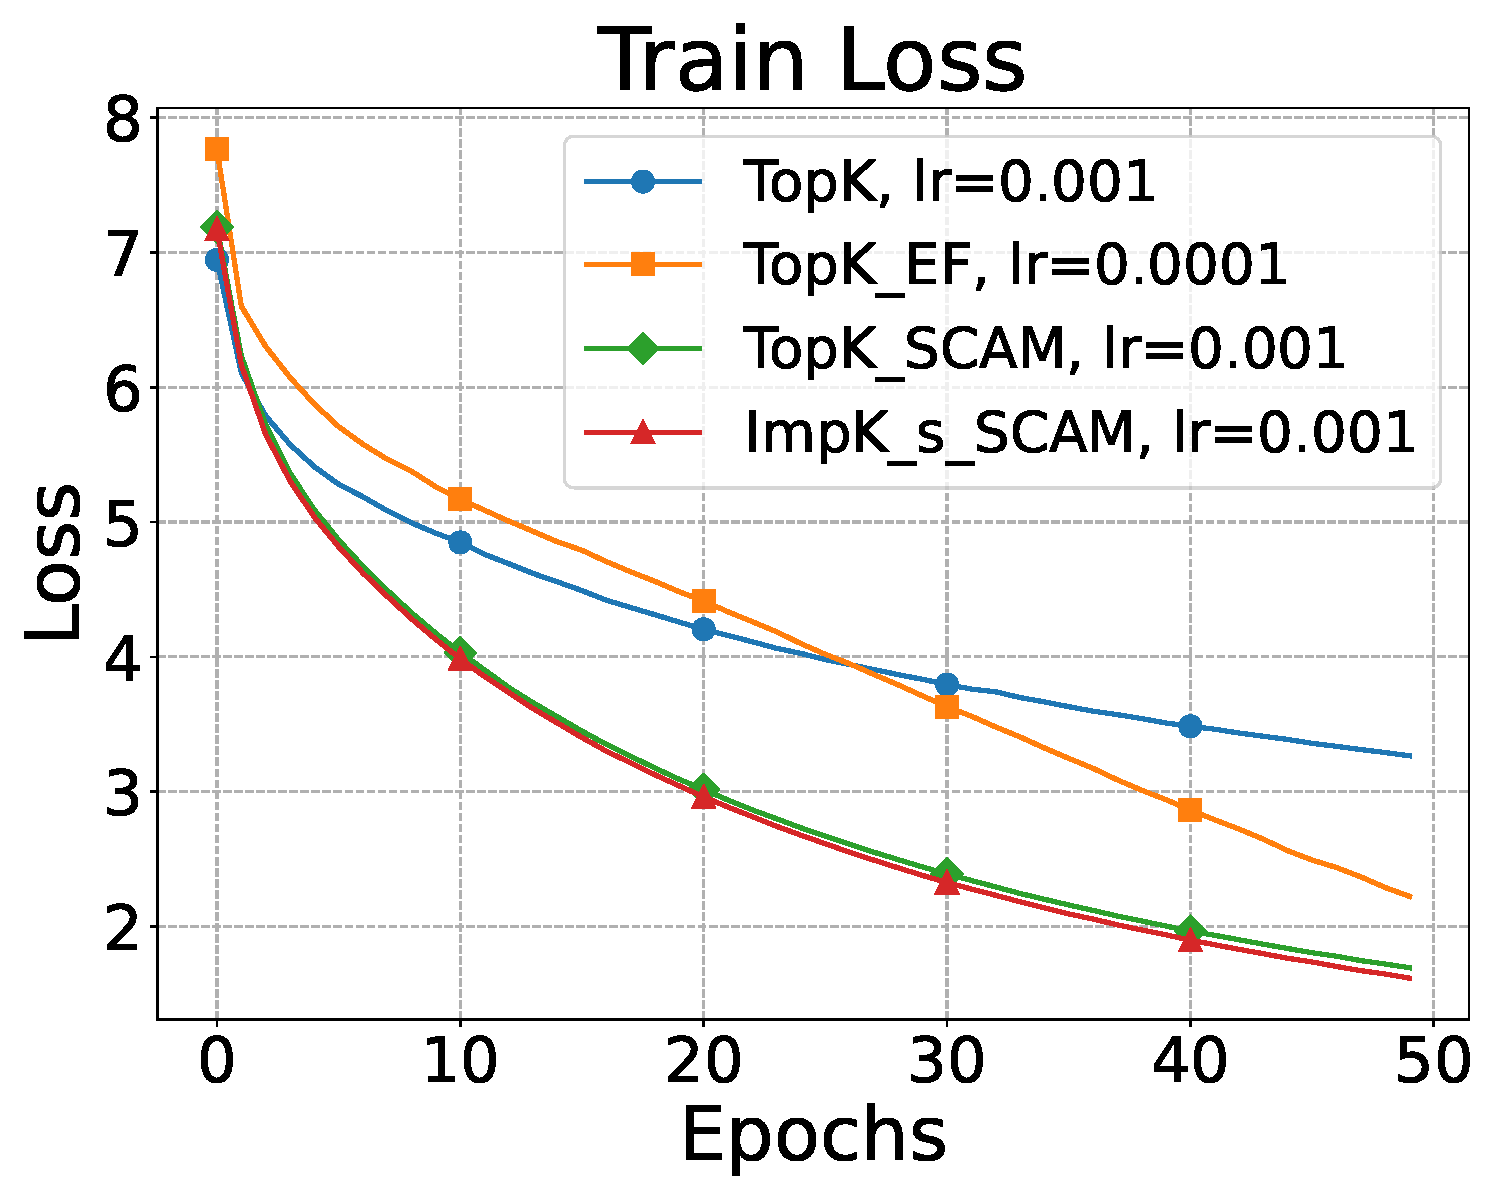
\includegraphics[width=\textwidth]{figures/gpt2/experiment2/Train Loss.pdf}
        \end{minipage}
        \begin{minipage}{0.45\textwidth}
            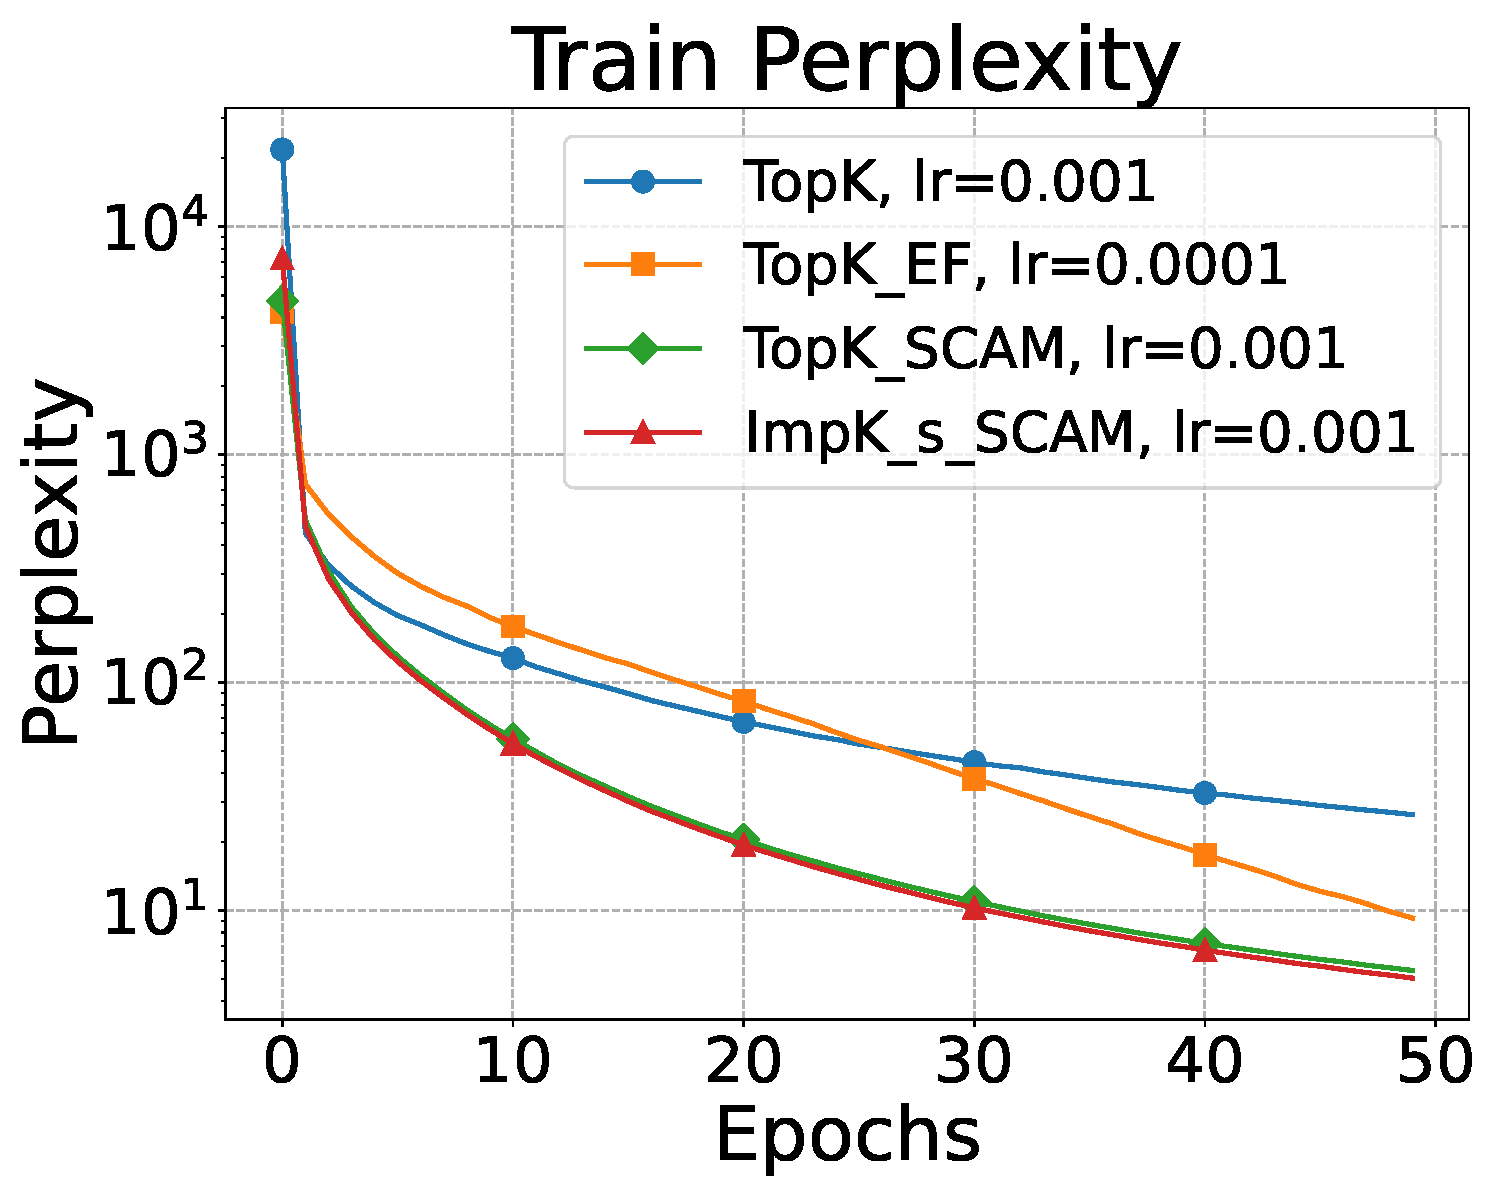
\includegraphics[width=\textwidth]{figures/gpt2/experiment2/Train Perplexity.pdf}
        \end{minipage}
        \begin{minipage}{0.45\textwidth}
            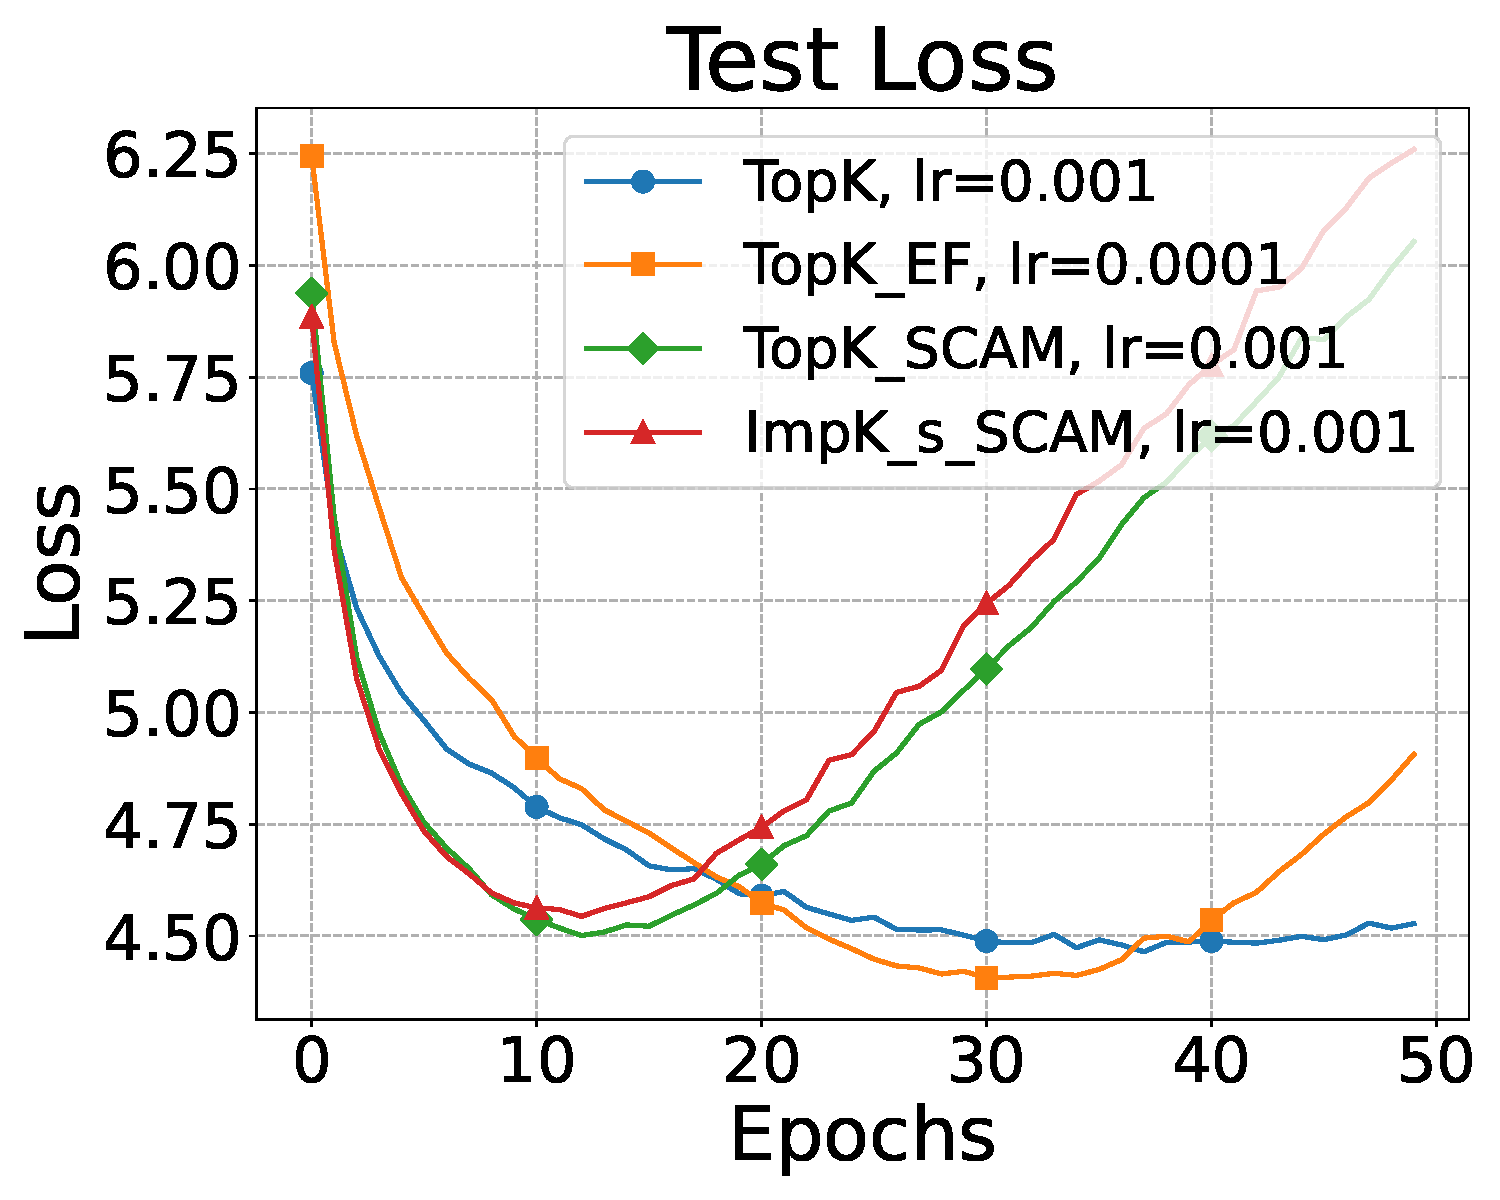
\includegraphics[width=\textwidth]{figures/gpt2/experiment2/Test Loss.pdf}
        \end{minipage}
        \begin{minipage}{0.45\textwidth}
            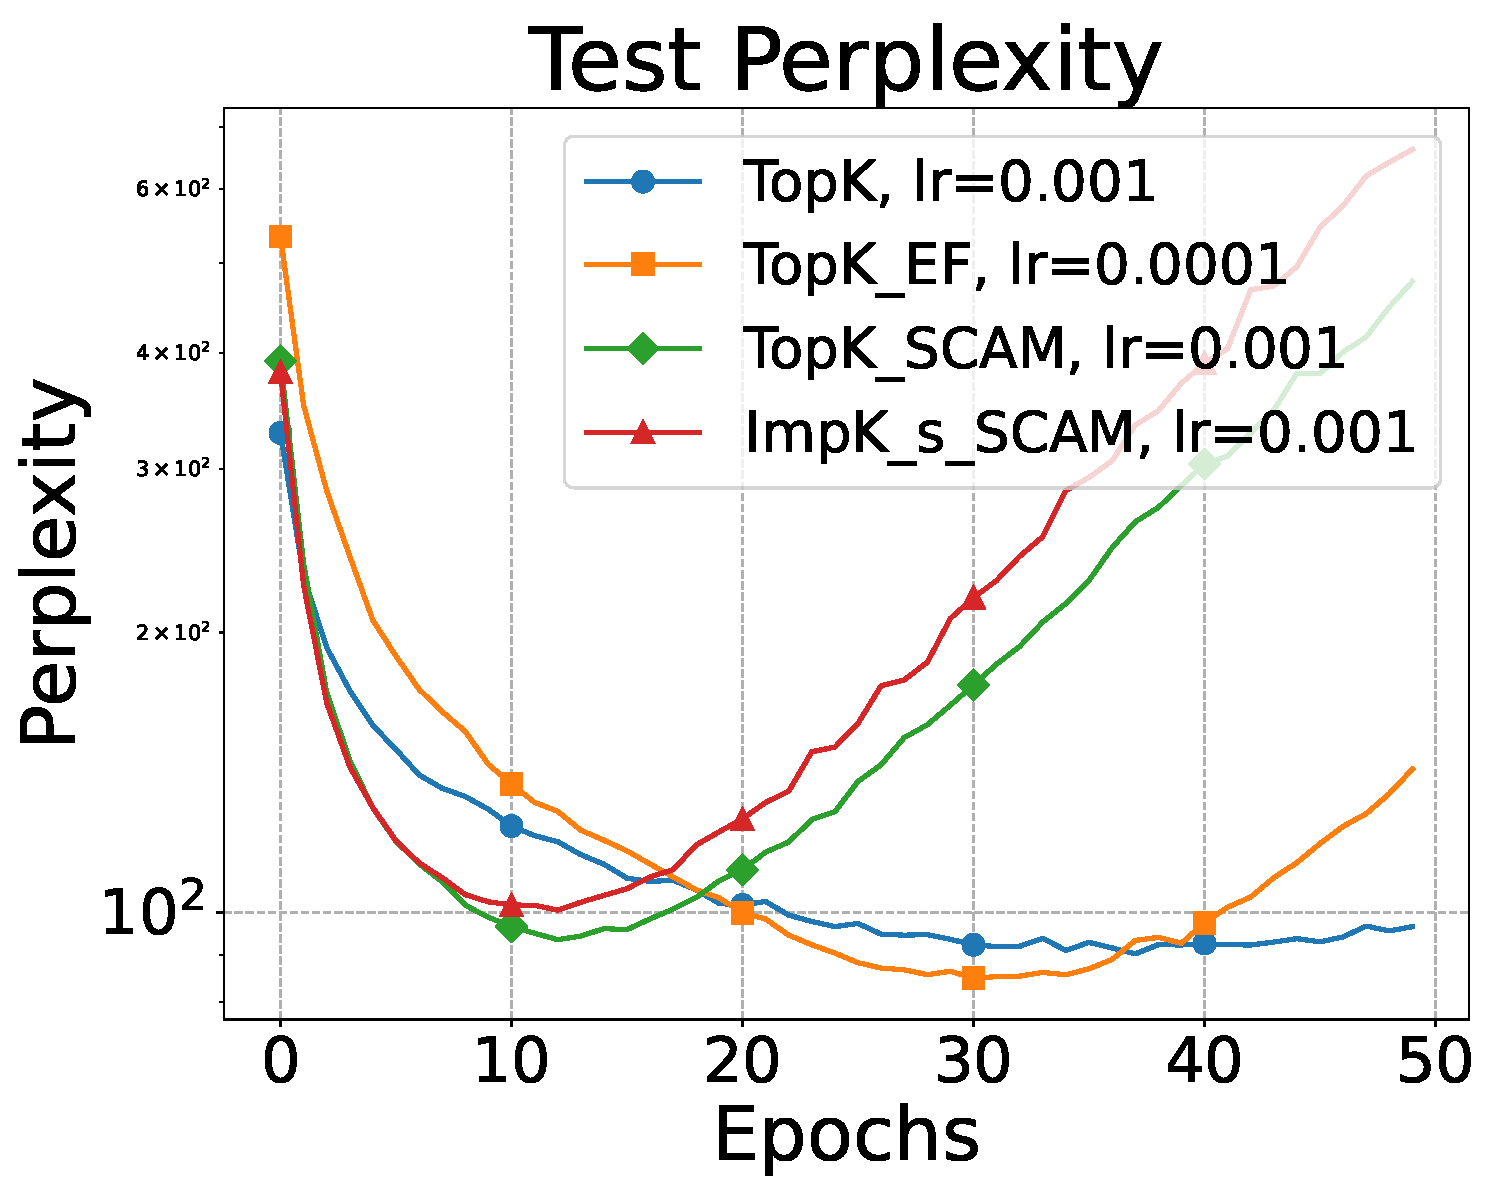
\includegraphics[width=\textwidth]{figures/gpt2/experiment2/Test Perplexity.pdf}
        \end{minipage}
        \caption{Сравнение производительности между предложенным методом SCAM $\impk_s$ и вариациями $\topk$ в процессе обучения GPT-2 на WikiText2.}
    \end{figure}

    Методы SCAM демонстрируют превосходство. Разница между SCAM $\impk_s$ и SCAM $\topk$ не столь выражена, но SCAM $\impk_s$ все же показывает лучшие результаты. Важным наблюдением является то, что на тестовом наборе данных заметно переобучение. Однако можно сделать вывод, что эта проблема возникает из-за недостаточного размера обучающего набора данных, и, вероятно, она уменьшится с увеличением размера обучающего набора данных. Поэтому в данном контексте следует сосредоточиться на кривых обучения.

    Этот эксперимент демонстрирует, что метод SCAM может быть также применен к архитектурам трансформеров, что особенно актуально в свете достижений в области больших языковых моделей.
